\chapter{Apéndice B: Herramientas Computacionales}
A continuación se presentarán las diferentes herramientas y metodologías a utilizar para desarrollar este trabajo.
\section{Metodologías}
Una metodología de trabajo se define como un conjunto de procesos estandarizados que facilitan el logro de objetivos particulares. En este caso nuestra metodología debe estar enfocada a lograr la minería de datos de forma eficiente.
A continuación se presentan diferentes metodologías conocidas para lograr nuestros objetivos.
\subsection{CRISP-DM}
Procedimiento que consiste en el descubrimiento de información valiosa a través del entendimiento del negocio constante y la evaluación de los resultados. Es un proceso cíclico de descubrimiento de la información. Actualmente es el proceso más utilizado para los estudios asociados al \textit{Data Mining}\cite{crispol,crispol2,crispol3}. En la Figura~\ref{fig:crisp} se señala el procedimiento.
\begin{figure}[H]
  \centering
    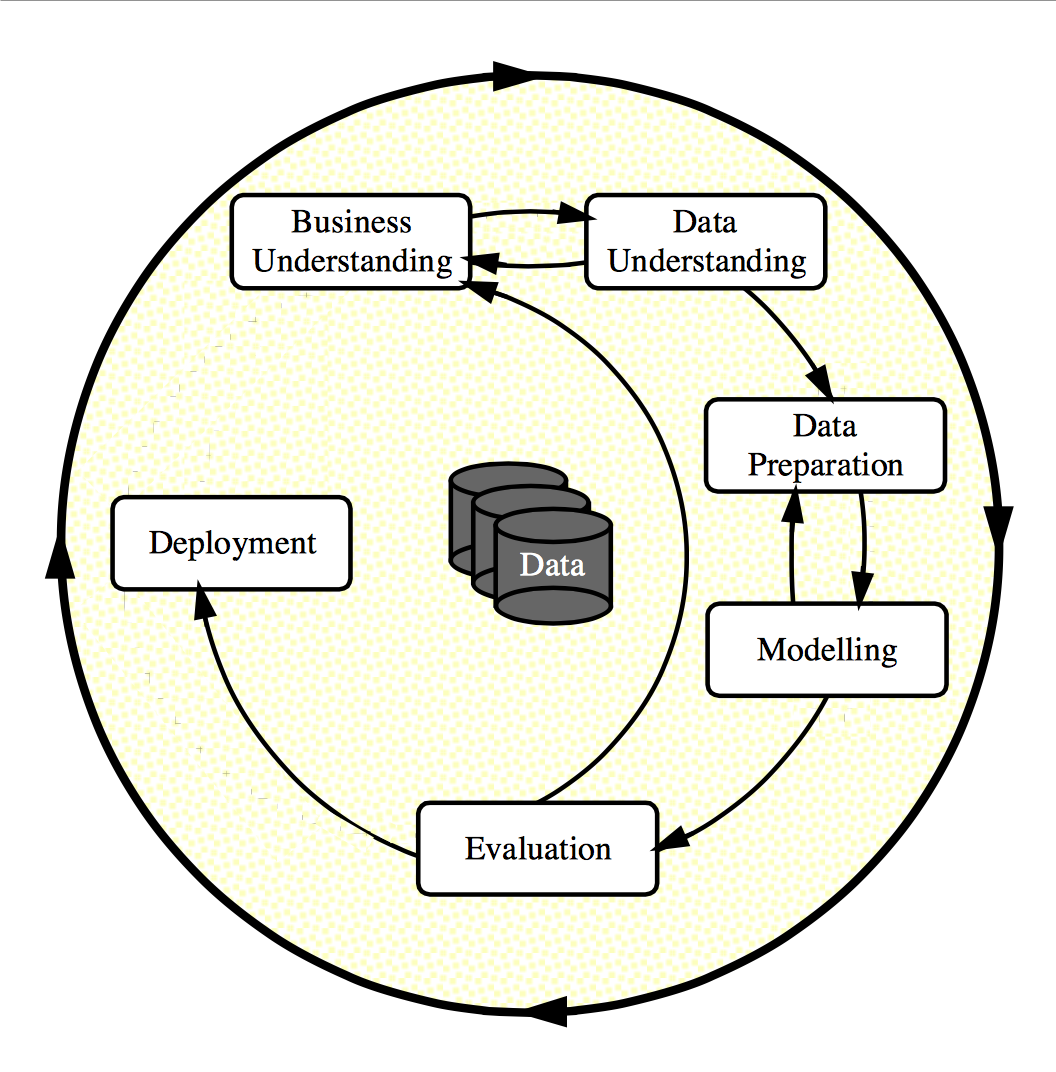
\includegraphics[width=0.5\textwidth]{Figuras/crisp-process}
      \caption{Procedimiento de \textit{\textbf{CR}oss \textbf{I}ndustry \textbf{S}tandard \textbf{P}rocess for \textbf{D}ata \textbf{M}ining}\cite{crisp}}
    \label{fig:crisp}
\end{figure}
\subsection{KDD/SEMMA}
Procedimiento que consiste en el descubrimiento de información útil dentro de colección de datos de información utilizando \textit{Data Mining}. El procedimiento se describe en la Figura~\ref{fig:kdd}.
\begin{figure}[H]
  \centering
    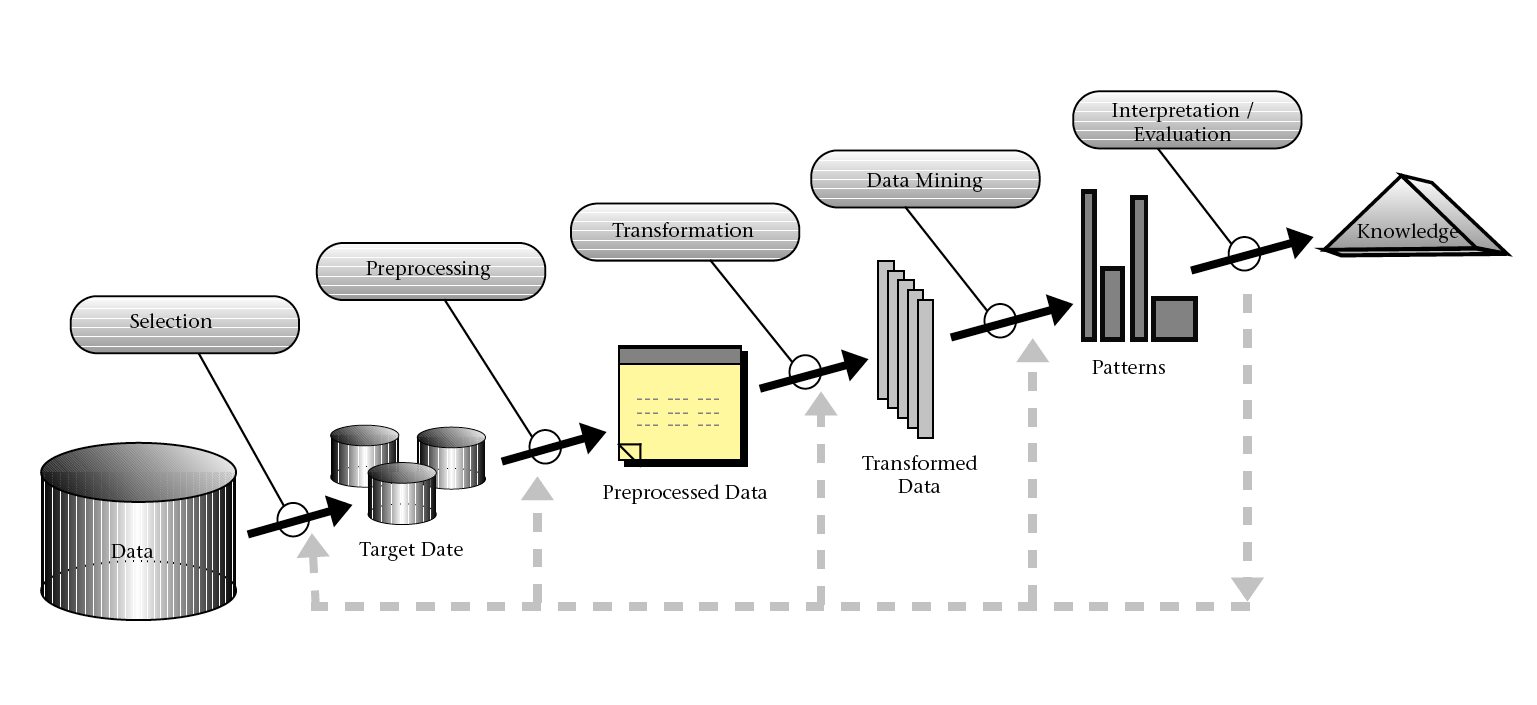
\includegraphics[width=0.8\textwidth]{Figuras/kdd-process}
      \caption{Procedimiento de \textit{Knowledge Discovery in Databases}\cite{kdd}}
    \label{fig:kdd}
\end{figure}

\subsection{Herramientas de Minería de Datos}
El problema que queremos resolver involucra clasificación y \textit{clustering} de la información, por tanto, es necesario uso de herramientas de \textit{Machine Learning} y Estadística\cite{barber}.
\newline
A continuación se presentan las diferentes opciones utilizadas en las literaturas consultadas sobre \textit{Educational Data Mining(EDM)}\cite{EDMSurv} y una breve descripción de estos:
\begin{description}
  \item[Decision Tree Learning] \hfill \\
  Modelo de predicción basado en árboles de decisiones que entrega las clasificaciones de una forma clara y sencilla.
  \item[Hierarchical Clustering] \hfill \\
  Modelo de predicción basado en la búsqueda de \textit{clusters} con relaciones jerárquicas entre ellos.
  \item[Logistic Regression] \hfill \\
  Modelo probabilístico capas de clasificar en variables discretas y no necesariamente continuas.
    \item[Linear/Multiple Regression] \hfill \\
  Modelo probabilístico que busca establecer una relación entre dos vectores.
  \item[K-means Clustering] \hfill \\
  Método de \textit{clustering} que consiste que busca particionar $n$ observaciones en $k$ \textit{clusters} utilizando la distancia promedio entre las observaciones.
  \item[Naive Bayes] \hfill \\
  Clasificador estadístico que asume independencia en las variables para lograr clasificar las observaciones en diferentes categorías.
  \item[Support Vector Machine] \hfill \\
  Método que busca particionar las observaciones utilizando hiperplanos para lograr el \textit{clustering} de estos mismos.
  \item[Artificial Neural Networks] \hfill \\
  Método de predicción que asimila a la función biologica del cerebro, es decir, se compone de varios nodos interconectados que se asemejan a las neuronas para lograr clasificar información.
\end{description}
\section{Herramientas Computacionales}
A continuación se presentará el 'software' que será utilizado para lograr los objetivos del trabajo.
\subsection{R-project\cite{rproject}}
R es un software que se utiliza para estadística y para graficar los resultados obtenidos. Es sencillo de utilizar, sin embargo no es la mejor opción cuando se requieren manejar demasiados datos. 
Como IDE utilizaremos R Studio, cuya  ventaja es la facilidad de su manejo incluso con bastante cantidad de ejemplos.
\subsection{Python Anaconda Package\cite{python}}
Python es un lenguaje de programación cuyo objetivo es generar una sintaxis que permita un código legible. Es un lenguaje de programación multiparadigma, es decir, soporta orientación tanto a objetos como programación imperativa y, en menor medida, programación funcional.
Lo bueno de este lenguaje de programación es que tiene mucho potencial, y en consecuencia, facilita el pre-procesamiento de los datos.
Se utilizará un paquete open-source llamado Anaconda que recopila los módulos necesarios para trabajar con Estadística y Aprendizaje Automático.
\subsection{WEKA\cite{weka}}
WEKA es una plataforma de software para el aprendizaje automático y la minería de datos escrito en Java.
El plus de este software es la interfaz gráfica que presenta y su facilidad de uso. Además, al igual que Python, WEKA es open-source, es decir, gratis. 
\subsection{Apache Hadoop\cite{hadoop}}
Al hablar de Hadoop señalamos el stack de software que desarrolló Apache para trabajar con procesamiento paralelo y mucha información. Normalmente el stack consiste en HDFS, YARN, Hive, Pig, Spark, HBase, MapReduce, Kafka y Mahout.